%note: don't split this document up with include{...}

\section{DFAFramework}

\subsection{Klassendiagramm}
\begin{figure}[htbp] 
	\centering
	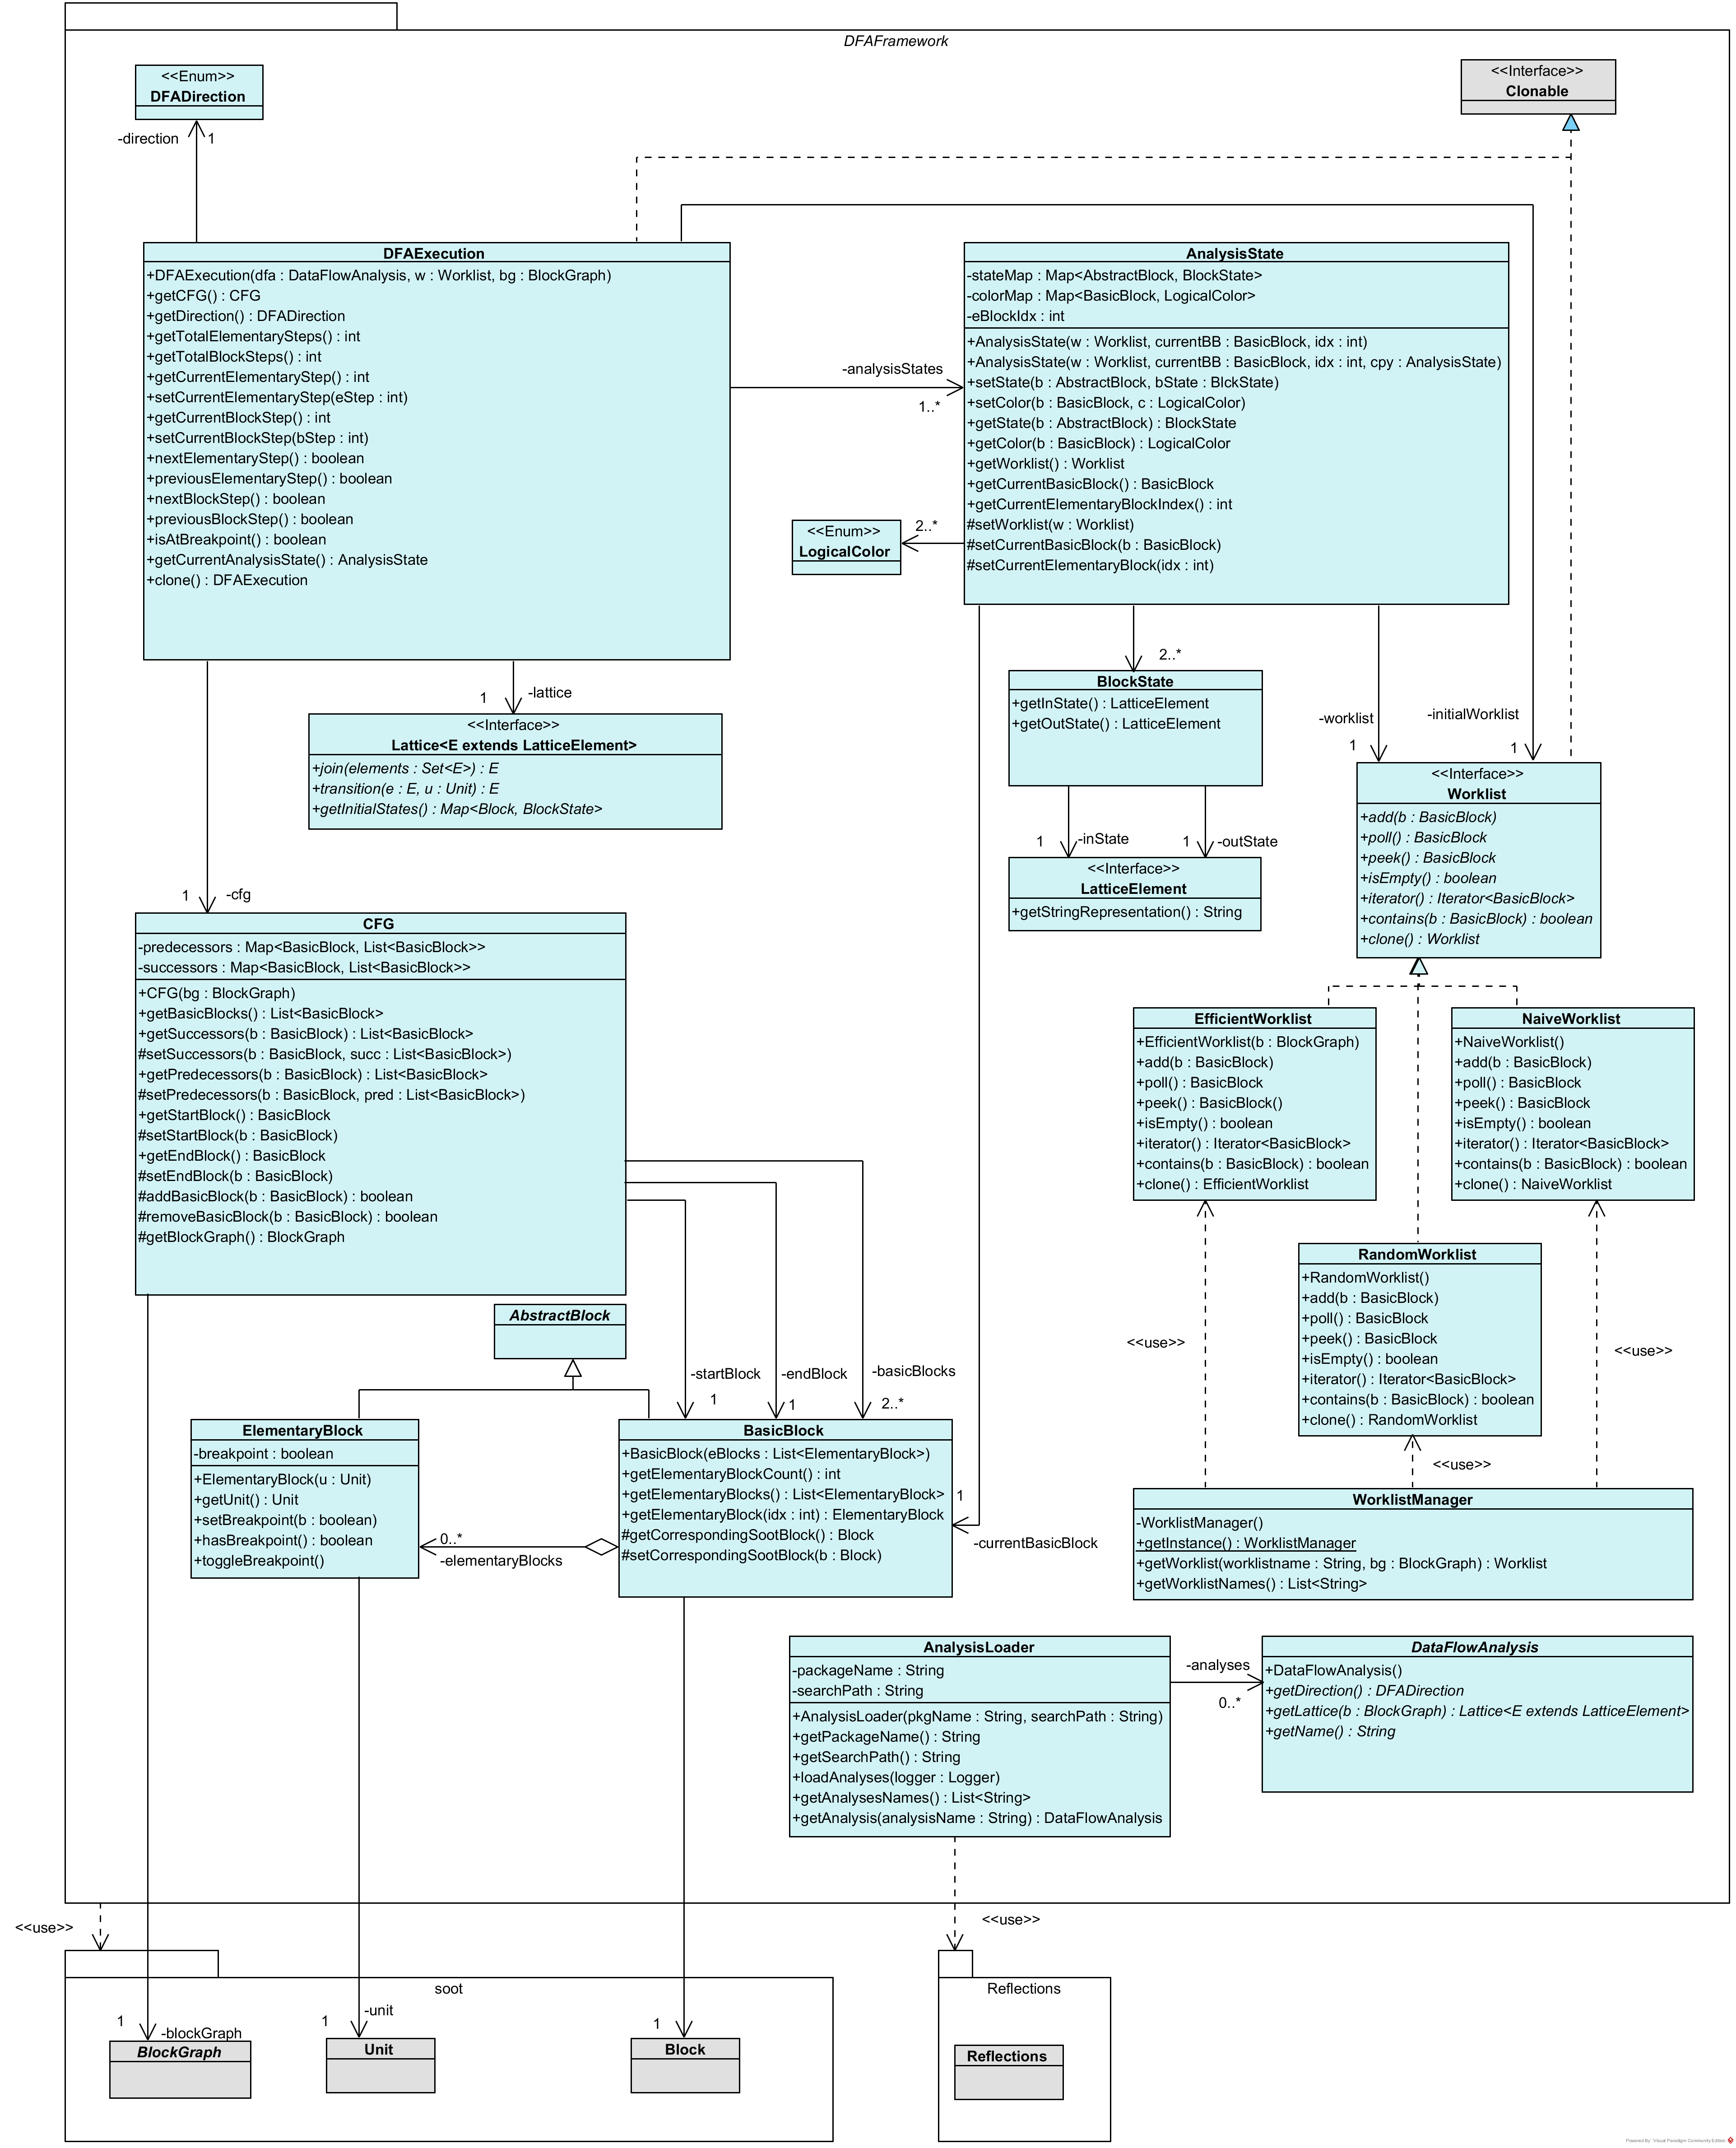
\includegraphics[width=1\textwidth]{Klassenuebersicht/DFAFramework/DFAFramework}
	\caption{Klassendiagramm des DFAFramework}
	\label{fig:DFAFreamework}
\end{figure}

%\newpage

Das DFAFramework ist für die Ausführung von Datenflussanalysen zuständig.
Weiter übernimmt das DFAFramework das Laden von Datenflussanalysen von einem festgelegten Speicherort.

Für die Ausführung von Datenflussanalysen ist die Klasse \inlinecode{DFAExecution} zentral.
Diese kann eine Datenflussanalyse für ein gegebenes \inlinecode{DataFlowAnalysis}-Objekt und einen gegebenen \inlinecode{BlockGraph} (\inlinecode{soot.toolkits.graph.BlockGraph}) vorberechnen.
Nach der Vorberechnung kann dann der aktuelle Analyseschritt mittels \inlinecode{nextElementaryStep()}, \inlinecode{previousElementaryStep()}, \inlinecode{setCurrentElementaryStep(stepNum : int)} und \inlinecode{getCurrentElementaryStep() : int} zeilenweise beliebig eingestellt bzw. abgefragt werden. 
Analog zu zeilenweisen Schritten können auch blockweise Schritte mittels \inlinecode{nextBlockStep()}, \inlinecode{previousBlockStep()}, \inlinecode{setCurrentBlockStep(step : int)} und \inlinecode{getCurrentBlockStep() : int} eingestellt und abgefragt werden.
Zudem kann mit \inlinecode{getCurrentAnalysisState() : AnalysisState} zu jedem Zeitpunkt der aktuelle Analysezustand erfragt werden.
Ein \inlinecode{AnalysisState} speichert dabei für jeden \inlinecode{AbstractBlock} (also sowohl für \inlinecode{ElementaryBlock}s als auch \inlinecode{BasicBlock}s) den aktuellen In- und Out-State, den aktuellen Zustand der \inlinecode{Worklist} sowie bei welchem \inlinecode{ElementaryBlock} bzw. \inlinecode{BasicBlock} sich die Analyse aktuell befindet.

Das Interface \inlinecode{Worklist} sowie die implementierenden Klassen \inlinecode{EfficientWorklist}, \inlinecode{NaiveWorklist} und \inlinecode{RandomWorklist} legen die Analysereihenfolge der einzelnen \inlinecode{BasicBlock}s fest und setzen damit das Entwurfsmuster der Strategie um.

Für die Implementierung konkreter Datenflussanalysen ist die Klasse \inlinecode{DataFlowAnalysis} essentiell.
Sie legt die Analyserichtung (\inlinecode{DFADirection}) sowie den Namen, unter dem eine Datenflussanalyse in der GUI auftaucht, fest.
Weiter bestimmt eine \inlinecode{DataFlowAnalysis} mittels \inlinecode{getLattice(blockGraph : BlockGraph) : Lattice} den für die Analyse verwendeten Verband.
Ein \inlinecode{Lattice} realisiert den Join-Operator mittels \inlinecode{join(elements : Set<LatticeElement>) : LatticeElement}.
Weiter gibt er zu allen unterstützten Expressions eine Übergangsfunktion mittels \inlinecode{transition(in : LatticeElement, unit : soot.Unit) : LatticeElement} an.
Schließlich gibt ein \inlinecode{Lattice} zu jedem Grundblock mittels \inlinecode{getInitialStates() : Map<Block, BlockState>} einen Initialzustand an. 
Mit den verschiedenen Implementierungen des Interfaces \inlinecode{Lattice} und den damit verbundenen Algorithmen für \inlinecode{join(elements : Set<LatticeElement>) : LatticeElement} und \inlinecode{transition(in : LatticeElement, unit : soot.Unit) : LatticeElement} kommt auch hier das Entwurfsmuster der Strategie fulminant zur Anwendung.

Ein \inlinecode{AnalysisLoader} ist für das Laden von Datenflussanalysen zuständig.
Mittels \inlinecode{loadAnalyses(logger : java.util.logging.Logger)} werden alle Unterklassen von \inlinecode{DataFlowAnalysis}, die an einem festgelegten Speicherort als .class-Dateien abgelegt sind, geladen.
Die Namen der geladenen Analysen können dann mit \inlinecode{getAnalysesNames() : List<String>} abgefragt werden.
Weiter kann mit \inlinecode{getAnalysis(analysisName : String) : DataFlowAnalysis} ein \inlinecode{DataFlowAnalysis}-Objekt über seinen Namen ermittelt werden.

\newpage

\subsection{Klassenbeschreibung}

\class{abstract DataFlowAnalysis}
\inlinecode{DataFlowAnalysis} ist die abstrakte Basisklasse für alle konkreten Datenflussanalysen.
Jede \inlinecode{DataFlowAnalysis} legt ihren Namen, die Richtung der Analyse sowie den verwendeten Verband fest.

\paragraph*{Konstruktoren} 
\begin{itemize}
	\item \ctor{DataFlowAnalysis}{}{public}{
	Instanziiert eine \inlinecode{DataFlowAnalysis}.
	}
\end{itemize}

\paragraph*{Methoden}
\begin{itemize}
	\item \method{getDirection}{DFADirection}{}{public abstract}{
	Gibt die \inlinecode{DFADirection} der \inlinecode{DataFlowAnalysis} zurück.
	}
	\item \method{getLattice}{Lattice<E extends LatticeElement>}{b : BlockGraph}{public abstract}{
	Gibt den \inlinecode{Lattice} zurück, auf welchem die \inlinecode{DataFlowAnalysis} basiert.
	}
	\item \method{getName}{String}{}{public abstract}{
	Gibt den Namen der \inlinecode{DataFlowAnalysis} zurück.
	}
\end{itemize}

\class{AnalysisLoader}
Ein \inlinecode{AnalysisLoader} ist für das Laden von Datenflussanalysen zuständig.
Dazu werden mittels der Reflections-Library alle Subklassen von \inlinecode{DataFlowAnalysis} aus dem bei der Erzeugung des \inlinecode{AnalysisLoader}s per Namen übergebenen Package geladen (siehe \inlinecode{loadAnalyses()}).

\paragraph*{Attribute}
\begin{itemize}
	\item \attr{analyses}{List<DataFlowAnalysis>}{private}{
	Die Liste aller implementierten und geladenen \inlinecode{DataFlowAnalysis}'.
	}
	\item \attr{packageName}{String}{private}{
	Der Name des Packages, in welchem sich die implementierten \inlinecode{DataFlowAnalysis}' befinden.
	}
	\item \attr{searchPath}{String}{private}{
	Der Pfad zu dem Ordner, in dem sich die implementierten \inlinecode{DataFlowAnalysis}' befinden.
	}
\end{itemize}

\paragraph*{Konstruktoren} 
\begin{itemize}
	\item \ctor{AnalysisLoader}{pkgName : String, searchPath : String}{public}{
	Instanziiert einen \inlinecode{AnalysisLoader}, welcher die implementierten \inlinecode{DataFlowAnalysis}' aus dem Package mit dem übergebenen Namen aus dem durch \inlinecode{searchPath} angegeben Ordner lädt.
	}
\end{itemize}

\paragraph*{Methoden}
\begin{itemize}
	\item \method{getPackageName}{String}{}{public}{
	Gibt \inlinecode{pkgName} zurück.
	}
	\item \method{loadAnalyses}{void}{logger : Logger}{public}{
	Lädt mit Hilfe des übergebenen Loggers alle implementierten \inlinecode{DataFlowAnalysis}' aus dem Package mit Name \inlinecode{pkgName}.
	}
	\item \method{getAnalysesNames}{List<String>}{}{public}{
	Gibt die Liste der Namen aller implementierten und geladenen \inlinecode{DataFlowAnalysis}' zurück
	}
	\item \method{getAnalysis}{DataFlowAnalysis}{analysisName : String}{public}{
	Gibt die \inlinecode{DataFlowAnalysis} zurück, welche den übergebenen Namen hat, sofern eine solche implementiert und geladen ist.
	}
\end{itemize}

\class{enum DFADirection}
Eine \inlinecode{DFADirection} gibt die Richtung einer Datenflussanalyse an.
Dabei gibt es die Richtungen \inlinecode{FORWARD} und \inlinecode{BACKWARD}.

\class{interface Lattice<E extends LatticeElement>}
Ein \inlinecode{Lattice} repräsentiert einen Verband, der für Datenflussanalysen verwendet wird.
Ein \inlinecode{Lattice} legt die Join-Operation fest, die bestimmt, wie mehrere \inlinecode{LatticeElement}s (\inlinecode{E}) zusammengeführt werden.
Weiter legt ein \inlinecode{Lattice} die Übergangsfunktionen fest, die bestimmt, wie ein \inlinecode{LatticeElement} von einer \inlinecode{soot.Unit} in ein neues \inlinecode{LatticeElement} überführt wird.
Schließlich bestimmt ein \inlinecode{Lattice} noch den Initialzustand (In- und Out-State) jedes \inlinecode{Block}s des der Analyse zugrunde liegenden \inlinecode{BlockGraph}s.
Damit setzt das Interface \inlinecode{Lattice} das Entwurfsmuster der Strategie um. 

\paragraph*{Methoden}
\begin{itemize}
	\item \method{join}{E}{elements : Set<E>}{public abstract}{
	Führt die Join-Operation dieses Verbands auf den übergebenen \inlinecode{LatticeElement}s aus.
	}
	\item \method{transition}{E}{e : E, u : Unit}{public abstract}{
	Führt die Übergangsfunktion, für die übergebene \inlinecode{Unit} auf dem übergebenen \inlinecode{LatticeElement} aus. 
	}
	\item \method{getInitialStates}{Map<Block, BlockState>}{}{public abstract}{
	Gibt eine \inlinecode{Map} zurück, die jedem \inlinecode{Block} einen initialen \inlinecode{BlockState} zuordnet.
	}
\end{itemize}

\class{interface LatticeElement}
Ein \inlinecode{LatticeElement} repräsentiert ein Element eines Verbandes (\inlinecode{Lattice}).
In- und Out-States von \inlinecode{AbstractBlock}s sind jeweils \inlinecode{LatticeElement}s (siehe \inlinecode{BlockState}).


\paragraph*{Methoden}
\begin{itemize}
	\item \method{getStringRepresentation}{String}{}{public abstract}{
	Gibt eine String-Repräsentation des \inlinecode{LatticeElement}s zurück.
	}
\end{itemize}

\class{DFAExecution}
Eine \inlinecode{DFAExecution} ist eine Datenflussanalyse in Ausführung. 
Beim Erzeugen eines neuen \inlinecode{DFAExecution}-Objekts wird die Datenflussanalyse vorberechnet. 
Danach kann der Zustand der Analyse zu beliebigen Zwischenschritten abgefragt werden.
Es wird zwischen Zeilenschritten und Blockschritten unterschieden.
Der aktuelle Blockschritt kann mit den Methoden \inlinecode{getCurrentBlockStep() : int} und \inlinecode{setCurrentBlockStep(bStep : int)} abgefragt bzw. gesetzt werden.
Analog kann mittels \inlinecode{getCurrentElementaryStep() : int} und \inlinecode{setCurrentElementaryStep(eStep : int)} der aktuelle Zeilenschritt abgefragt oder eingestellt werden.
Weiter kann mit \inlinecode{nextElementaryStep() : boolean} und \inlinecode{previousElementaryStep() : boolean} zeilenweise, sowie mit \inlinecode{nextBlockStep() : boolean} und \inlinecode{previousBlockStep() : boolean} blockweise durch die Analyse navigiert werden.

\paragraph*{Attribute}
\begin{itemize}
	\item \attr{initialWorklist}{Worklist}{private}{
	Die \inlinecode{Worklist}, welche für die Ausführung der Datenflussanalyse verwendet wird.
	}
	\item \attr{analysisStates}{List<AnalysisState>}{private}{
	Liste der vorberechneten \inlinecode{AnalysisState}s.
	}
	\item \attr{lattice}{Lattice<E extends LatticeElement>}{private}{
	Der \inlinecode{Lattice}, also der Verband, welcher der Datenflussanalyse zugrunde liegt.
	}
	\item \attr{cfg}{CFG}{private}{
	Der \inlinecode{CFG}, also der Kontrollflussgraph, auf welchem die Datenflussanalyse ausgeführt wird.
	}
\end{itemize}

\paragraph*{Konstruktoren} 
\begin{itemize}
	\item \ctor{DFAExecution}{dfa : AbstractDataFlowAnalysis, w : Worklist, bg : BlockGraph}{public}{
	Erzeugt eine \inlinecode{DFAExecution} mit folgenden Parametern:
	\begin{itemize}[topsep=-8pt] \setlength\itemsep{-12pt}
		\item eine \inlinecode{AbstractDataFlowAnalysis}, welche angibt, welche Art der Datenflussanalyse ausgeführt wird
		\item eine Instanz, welche das Interface \inlinecode{Worklist} implementiert und den Worklistalgorithmus enthält, der zur Ausführung der Datenflussanalyse verwendet wird
		\item ein \inlinecode{BlockGraph}, der dem Kontrollflussgraphen des zu analysierenden Codes entspricht 
	\end{itemize}
	Ein \inlinecode{CFG} wird aus dem \inlinecode{BlockGraph} erstellt. 
	Alle Schritte der Datenflussanalyse	werden vorberechnet.
	}
\end{itemize}

\paragraph*{Methoden}
\begin{itemize}
	\item \method{getCFG}{CFG}{}{public}{
	Gibt den \inlinecode{CFG} zurück, auf dem die Datenflussanalyse ausgeführt wird.
	}
	\item \method{getDirection}{DFADirection}{}{public}{
	Gibt die Richtung der Datenflussanalyse zurück.
	}
	\item \method{getTotalElementarySteps}{int}{}{public}{
	Gibt die Gesamtanzahl der Zeilenschritte in der vorberechneten Analyse zurück.
	}
	\item \method{getTotalBlockSteps}{int}{}{public}{
	Gibt die Gesamtanzahl der Blockschritte in der vorberechneten Analyse zurück.
	}
	\item \method{getCurrentElementaryStep}{int}{}{public}{
	Gibt den aktuellen Zeilenschritt zurück.
	}
	\item \method{setCurrentElementaryStep}{void}{eStep : int}{public}{
	Setzt den aktuellen Zeilenschritt auf \inlinecode{eStep}. 
	Der Zustand der Analyse springt also an den übergebenen Zeilenschritt.
	Dabei ändert sich auch der aktuelle Blockschritt konsistent zum Zeilenschritt.
	}
	\item \method{getCurrentBlockStep}{int}{}{public}{
	Gibt den aktuellen Blockschritt zurück.
	}
	\item \method{setCurrentBlockStep}{void}{bStep : int}{public}{
	Setzt den aktuellen Blockschritt auf \inlinecode{bStep}. 
	Der Zustand der Analyse springt also an die übergebene Stelle.
	Dabei ändert sich auch der aktuelle Zeilenschritt konsistent zum Blockschritt.
	}
	\item \method{nextElementaryStep}{boolean}{}{public}{
	Inkrementiert den aktuellen Zeilenschritt um eins. 
	Die Analyse springt also zur nächsten Zeile.
	Dabei ändert sich ggf. der aktuelle Blockschritt konsistent zum Zeilenschritt.
	Gibt zurück, ob das Springen zur nächsten Zeile erfolgreich war.
	}
	\item \method{previousElementaryStep}{boolean}{}{public}{
	Dekrementiert den aktuellen Zeilenschritt um eins. 
	Die Analyse springt also zur vorherigen Zeile.
	Dabei ändert sich ggf. der aktuelle Blockschritt konsistent zum Zeilenschritt.
	Gibt zurück, ob das Springen zur vorherigen Zeile erfolgreich war.
	}
	\item \method{nextBlockStep}{boolean}{}{public}{
	Inkrementiert den aktuellen Blockschritt um eins. 
	Die Analyse springt also zum nächsten Block.
	Dabei ändert sich ggf. der aktuelle Zeilenschritt konsistent zum Blockschritt.
	Gibt zurück, ob das Springen zum nächsten Block erfolgreich war.
	}
	\item \method{previousBlockStep}{boolean}{}{public}{
	Dekrementiert den aktuellen Blockschritt um eins. 
	Die Analyse springt also zum vorherigen Block.
	Dabei ändert sich ggf. der aktuelle Zeilenschritt konsistent zum Blockschritt.
	Gibt zurück, ob das Springen zum vorherigen Block erfolgreich war.
	}
	\item \method{isAtBreakpoint}{boolean}{}{public}{
	Gibt zurück, ob sich in der Zeile, in der sich die Datenflussanalyse aktuell befindet, ein Breakpoint befindet.	
	}
	\item \method{getCurrentAnalysisState}{AnalysisState}{}{public}{
	Gibt den aktuellen Zustand der Analyse zurück.	
	}
	\item \method{clone}{DFAExecution}{}{public}{
	Gibt eine geklonte Instanz der \inlinecode{DFAExecution} zurück.
	}
\end{itemize}

\class{AnalysisState}
Ein \inlinecode{AnalysisState} repräsentiert einen Zustand einer Datenflussanalyse in einem Analyseschritt.
Dies beinhaltet den aktuellen Grundblock (\inlinecode{BasicBlock}) sowie die aktuelle Zeile darin (\inlinecode{ElementaryBlock}).
Jedem \inlinecode{AbstractBlock} (also jedem \inlinecode{BasicBlock} und jedem \inlinecode{ElementaryBlock}) wird ein \inlinecode{BlockState} zugeordnet.
Weiter wird der aktuelle Zustand der \inlinecode{Worklist} gespeichert.

\paragraph*{Attribute}
\begin{itemize}
	\item \attr{stateMap}{Map<AbstractBlock, BlockState>}{private} {
	Eine \inlinecode{Map}, welche jedem \inlinecode{BasicBlock} einen \inlinecode{BlockState} zuordnet, welcher den aktuellen In- und Out-State des Blocks repräsentiert.
	}
	\item \attr{colorMap}{Map<BasicBlock, LogicalColor>}{private}{
	Eine \inlinecode{Map}, welche jedem \inlinecode{BasicBlock} eine \inlinecode{LogicalColor} zuordnet.
	Dabei beschreibt eine \inlinecode{LogicalColor} den Zustand eines \inlinecode{BasicBlock}s im Bezug auf die Worklist (siehe \inlinecode{LogicalColor}).
	}
	\item \attr{worklist}{Worklist}{private}{
	Die aktuelle \inlinecode{Worklist}, welche die \inlinecode{BasicBlock}s enthält, die noch zu bearbeiten sind.
	}
	\item \attr{currentBasicBlock}{BasicBlock}{private}{
	Der \inlinecode{BasicBlock}, welcher im aktuellen Analysezustand bearbeitet wird.
	}
	\item \attr{eBlockIdx}{int}{private}{
	Der Zeilen-Index des im aktuellen Analysezustand bearbeiteten \inlinecode{ElementaryBlock}s.
	}
\end{itemize}

\paragraph*{Konstruktoren} 
\begin{itemize}
	\item \ctor{AnalysisState}{w : Worklist, currentBB : BasicBlock, idx : int}{public}{
	Erzeugt einen \inlinecode{AnalysisState} aus
	\begin{itemize}[topsep=-8pt] \setlength\itemsep{-12pt}
		\item einer \inlinecode{Worklist}, aus welcher durch Kopieren die \inlinecode{Worklist} des erzeugten \inlinecode{AnalysisState}s erstellt wird
		\item einem neuen aktuellen \inlinecode{BasicBlock}
		\item dem Zeilen-Index des neuen aktuellen \inlinecode{ElementaryBlock}s 
	\end{itemize}
	}
	\item \ctor{AnalysisState}{w : Worklist, currentBB : BasicBlock, idx : int, cpy : AnalysisState}{public}{
	Erzeugt einen \inlinecode{AnalysisState}, aus
	\begin{itemize}[topsep=-8pt] \setlength\itemsep{-12pt}
		\item einer \inlinecode{Worklist}, aus welcher durch Kopieren die \inlinecode{Worklist} des erzeugten \inlinecode{AnalysisState}s erstellt wird
		\item einem neuen aktuellen \inlinecode{BasicBlock}
		\item dem Zeilen-Index des neuen aktuellen \inlinecode{ElementaryBlock}s 
		\item einem \inlinecode{AnalysisState}, von dem das Mapping von \inlinecode{BasicBlock}s zu \inlinecode{BlockState}s übernommen wird
	\end{itemize}
	}
\end{itemize}

\paragraph*{Methoden}
\begin{itemize}
	\item \method{setState}{void}{b : AbstractBlock, bState : BlockState}{public}{
	Setzt den Zustand eines übergebenen \inlinecode{AbstractBlock}s auf den übergebenen \inlinecode{BlockState}.
	}
	\item \method{setColor}{void}{b : BasicBlock, c : LogicalColor}{public}{
	Setzt die \inlinecode{LogicalColor} eines übergebenen \inlinecode{BasicBlock}s.
	}
	\item \method{getState}{BlockState}{b : AbstractBlock}{public}{
	Gibt den aktuellen \inlinecode{BlockState} des übergebenen \inlinecode{AbstractBlock}s zurück.
	}
	\item \method{getColor}{LogicalColor}{b : BasicBlock}{public}{
	Gibt die aktuelle \inlinecode{LogicalColor} des übergebenen \inlinecode{BasicBlock}s zurück.
	}
	\item \method{getWorklist}{Worklist}{}{public}{
	Gibt die \inlinecode{Worklist} in diesem \inlinecode{AnalysisState} zurück.
	}
	\item \method{getCurrentBasicBlock}{BasicBlock}{}{public}{
	Gibt den aktuellen \inlinecode{BasicBlock} zurück.
	}
	\item \method{getCurrentElementaryBlock}{ElementaryBlock}{}{public}{
	Gibt den aktuellen \inlinecode{ElementaryBlock} zurück.
	}
	\item \method{getCurrentElementaryBlockIndex}{int}{}{public}{
	Gibt den Zeilen-Index des aktuellen \inlinecode{ElementaryBlock}s zurück.
	}
	\item \method{setWorklist}{void}{w : Worklist}{protected}{
	Setzt die übergebene \inlinecode{Worklist} als aktuelle \inlinecode{Worklist} dieses \inlinecode{AnalysisState}s.
	}
	\item \method{setCurrentBasicBlock}{void}{b : BasicBlock}{protected}{
	Setzt den übergebenen \inlinecode{BasicBlock} als den aktuellen \inlinecode{BasicBlock}.
	}
	\item \method{setCurrentElementaryBlock}{void}{idx : int}{protected}{
	Setzt den übergeben Index als Zeilen-Index des aktuellen \inlinecode{ElementaryBlock}s.
	}
\end{itemize}

\class{BlockState}
Ein \inlinecode{BlockState} fasst den In- und Out-State eines \inlinecode{AbstractBlock}s zusammen.
Sowohl der In- und Out-State sind dabei jeweils ein \inlinecode{LatticeElement}.

\paragraph*{Attribute}
\begin{itemize}
	\item \attr{inState}{LatticeElement}{private}{
	Das \inlinecode{LatticeElement}, welches die Fakten darstellt, die bei Eingang in den \inlinecode{AbstractBlock} gelten, zu welchem dieser \inlinecode{BlockState} gehört.
	}
	\item \attr{outState}{LatticeElement}{private}{
	Das \inlinecode{LatticeElement}, welches die Fakten darstellt, die bei Ausgang aus dem \inlinecode{AbstractBlock} gelten, zu welchem dieser \inlinecode{BlockState} gehört.
	}
\end{itemize}

\paragraph*{Konstruktoren} 
\begin{itemize}
	\item \ctor{BlockState}{inState : LatticeElement, outState : LatticeElement}{public}{
	Instanziiert einen \inlinecode{BlockState}, welcher die übergebenen \inlinecode{LatticeElement}s als In- bzw Out-State hat.
	}
\end{itemize}

\paragraph*{Methoden}
\begin{itemize}
	\item \method{getInState}{LatticeElement}{}{public}{
	Gibt den \inlinecode{inState} zurück.
	}
	\item \method{getOutState}{LatticeElement}{}{public}{
	Gibt den \inlinecode{outState} zurück.
	}
\end{itemize}

\class{interface Worklist extends Cloneable}
Eine \inlinecode{Worklist} legt fest, welche \inlinecode{BasicBlock}s noch zu bearbeiten sind und in welcher Reihenfolge dies geschieht.
Von einer \inlinecode{Worklist} kann mittels \inlinecode{clone()} stets eine tiefe Kopie angefertigt werden. Das Interface \inlinecode{Worklist} entspricht dem Entwurfsmuster der Strategie.

\paragraph*{Methoden}
\begin{itemize}
	\item \method{add}{void}{b : BasicBlock}{public abstract}{
	Fügt den übergebenen \inlinecode{BasicBlock} zur \inlinecode{Worklist} hinzu.	
	}
	\item \method{poll}{BasicBlock}{}{public abstract}{
	Gibt den nächsten \inlinecode{BasicBlock} von der \inlinecode{Worklist} zurück und löscht diesen von der \inlinecode{Worklist}.
	}
	\item \method{peek}{BasicBlock}{}{public abstract}{
	Gibt den nächsten \inlinecode{BasicBlock} von der \inlinecode{Worklist} zurück, aber belässt diesen auf der \inlinecode{Worklist}.
	}
	\item \method{isEmpty}{boolean}{}{public abstract}{
	Gibt zurück, ob sich noch \inlinecode{BasicBlock}s auf der \inlinecode{Worklist} befinden (\inlinecode{false}) oder nicht (\inlinecode{true}).
	}
	\item \method{iterator}{Iterator<BasicBlock>}{}{public abstract}{
	Gibt einen \inlinecode{Iterator} über alle \inlinecode{BasicBlock}s auf der \inlinecode{Worklist} zurück.
	}
	\item \method{contains}{boolean}{b : BasicBlock}{public abstract}{
	Gibt zurück, ob sich der übergebene \inlinecode{BasicBlock} auf der \inlinecode{Worklist} befindet (\inlinecode{true}) oder nicht (\inlinecode{false}).
	}
	\item \method{getName}{String}{}{public abstract}{
	Gibt den Namen des in der \inlinecode{Worklist} verwendeten Worklistalgorithmus' zurück.
	}
	\item \method{clone}{Worklist}{}{public abstract}{
	Erstellt eine tiefe Kopie dieser \inlinecode{Worklist}.
	Insbesondere hat das Manipulieren der zurückgegebenen \inlinecode{Woklist} keinen Einfluss auf das der Kopie zugrunde liegende Objekt und umgekehrt.
	}
\end{itemize}

\class{EfficientWorklist implements Worklist}
Eine \inlinecode{EfficientWorklist} gibt die enthaltenen \inlinecode{BasicBlock}s bei der Abarbeitung mittels \inlinecode{peek()} und \inlinecode{poll()} in einer Reihenfolge zurück, die möglichst günstig für die Laufzeit (bzgl. der Schrittzahl) der Fixpunktiteration ist.

\paragraph*{Konstruktoren} 
\begin{itemize}
	\item \ctor{EfficientWorklist}{b : BlockGraph}{public}{
	Erzeugt eine leere \inlinecode{EfficientWorklist} aus einem gegebenen \inlinecode{BlockGraph}.
	}
\end{itemize}

\paragraph*{Methoden}
\begin{itemize}
	\item \method{add}{void}{b : BasicBlock}{public}{
	Fügt den übergebenen \inlinecode{BasicBlock} zur \inlinecode{EfficientWorklist} hinzu, falls er nicht schon enthalten ist.	
	}
	\item \method{poll}{BasicBlock}{}{public}{
	Gibt den nächsten \inlinecode{BasicBlock} von dieser \inlinecode{EfficientWorklist} zurück und entfernt ihn von dieser \inlinecode{EfficientWorklist}.
	Dabei wird der nächste \inlinecode{BasicBlock} so gewählt, dass die mittlere Laufzeit der Fixpunktiteration möglichst gering ist.
	}
	\item \method{peek}{BasicBlock}{}{public}{
	Gibt den nächsten \inlinecode{BasicBlock} von dieser \inlinecode{EfficientWorklist} zurück, aber belässt diesen auf der \inlinecode{EfficientWorklist}.
	Dabei wird der nächste \inlinecode{BasicBlock} so gewählt, dass die mittlere Laufzeit der Fixpunktiteration möglichst gering ist.
	}
	\item \method{isEmpty}{boolean}{}{public}{
	Gibt zurück, ob sich noch \inlinecode{BasicBlock}s auf dieser \inlinecode{EfficientWorklist} befinden (\inlinecode{false}) oder nicht (\inlinecode{true}).
	}
	\item \method{iterator}{Iterator<BasicBlock>}{}{public}{
	Gibt einen \inlinecode{Iterator} über alle \inlinecode{BasicBlock}s auf der \inlinecode{EfficientWorklist} zurück.
	}
	\item \method{contains}{boolean}{b : BasicBlock}{public}{
	Gibt zurück, ob sich der übergebene \inlinecode{BasicBlock} auf der \inlinecode{EfficientWorklist} befindet (\inlinecode{true}) oder nicht (\inlinecode{false}).
	}
	\item \method{clone}{EfficientWorklist}{}{public}{
	Gibt eine tiefe Kopie \inlinecode{EfficientWorklist} zurück.
	}
	\item \method{getName}{String}{}{public}{
	Gibt den Namen zurück, unter dem eine \inlinecode{EfficientWorklist} in der GUI angezeigt werden soll.
	}
\end{itemize}

\class{RandomWorklist implements Worklist}
Eine \inlinecode{RandomWorklist} gibt die enthaltenen \inlinecode{BasicBlock}s bei Abarbeitung mittels \inlinecode{peek()} und \inlinecode{poll()} in einer (pseudo-)zufälligen Reihenfolge zurück.

\paragraph*{Konstruktoren} 
\begin{itemize}
	\item \ctor{RandomWorklist}{}{public}{
	Erzeugt eine leere \inlinecode{RandomWorklist}.
	}
\end{itemize}

\paragraph*{Methoden}
\begin{itemize}
	\item \method{add}{void}{b : BasicBlock}{public}{
	Fügt den übergebenen \inlinecode{BasicBlock} zur \inlinecode{RandomWorklist} hinzu, falls er nicht schon enthalten ist.	
	}
	\item \method{poll}{BasicBlock}{}{public}{
	Gibt einen zufälligen \inlinecode{BasicBlock} von der \inlinecode{RandomWorklist} zurück und löscht diesen von der \inlinecode{RandomWorklist}.
	}
	\item \method{peek}{BasicBlock}{}{public}{
	Gibt einen zufälligen \inlinecode{BasicBlock} von der \inlinecode{RandomWorklist} zurück aber belässt diesen auf der \inlinecode{RandomWorklist}.
	}
	\item \method{isEmpty}{boolean}{}{public}{
	Gibt zurück, ob sich noch \inlinecode{BasicBlock}s auf der \inlinecode{RandomWorklist} befinden (\inlinecode{false}) oder nicht \inlinecode{true}.
	}
	\item \method{iterator}{Iterator<BasicBlock>}{}{public}{
	Gibt einen \inlinecode{Iterator} über alle \inlinecode{BasicBlock}s auf der \inlinecode{RandomWorklist} zurück.
	}
	\item \method{contains}{boolean}{b : BasicBlock}{public}{
	Gibt zurück, ob sich der übergebene \inlinecode{BasicBlock} auf der \inlinecode{RandomWorklist} befindet (\inlinecode{true}) oder nicht (\inlinecode{false}).
	}
	\item \method{clone}{RandomWorklist}{}{public}{
	Gibt eine tiefe Kopie dieser \inlinecode{RandomWorklist} zurück.
	}
	\item \method{getName}{String}{}{public}{
	Gibt den Namen zurück, unter dem eine \inlinecode{RandomWorklist} in der GUI angezeigt werden soll.
	}
\end{itemize}

\class{NaiveWorklist implements Worklist}
Eine \inlinecode{NaiveWorklist} gibt die enthaltenen \inlinecode{BasicBlock}s bei Abarbeitung mittels \inlinecode{peek()} und \inlinecode{poll()} der Reihenfolge zurück, in der sie hinzugefügt wurden.

\paragraph*{Konstruktoren} 
\begin{itemize}
	\item \ctor{NaiveWorklist}{}{public}{
	Erzeugt eine leere \inlinecode{NaiveWorklist}.
	}
\end{itemize}

\paragraph*{Methoden}
\begin{itemize}
	\item \method{add}{void}{b : BasicBlock}{public}{
	Fügt den übergebenen \inlinecode{BasicBlock} zur \inlinecode{NaiveWorklist} hinzu, falls er nicht schon enthalten ist.	
	}
	\item \method{poll}{BasicBlock}{}{public}{
	Gibt den nächsten \inlinecode{BasicBlock} von der \inlinecode{NaiveWorklist} zurück und löscht diesen von der \inlinecode{NaiveWorklist}.
	}
	\item \method{peek}{BasicBlock}{}{public}{
	Gibt den nächsten \inlinecode{BasicBlock} von der \inlinecode{NaiveWorklist} zurück, aber belässt diesen auf der \inlinecode{NaiveWorklist}.
	}
	\item \method{isEmpty}{boolean}{}{public}{
	Gibt zurück, ob sich noch \inlinecode{BasicBlock}s auf der \inlinecode{NaiveWorklist} befinden (\inlinecode{false}) oder nicht (\inlinecode{true}).
	}
	\item \method{iterator}{Iterator<BasicBlock>}{}{public}{
	Gibt einen Iterator über alle \inlinecode{BasicBlock}s auf der \inlinecode{NaiveWorklist} zurück.
	}
	\item \method{contains}{boolean}{b : BasicBlock}{public}{
	Gibt zurück, ob sich der übergebene \inlinecode{BasicBlock} auf der \inlinecode{NaiveWorklist} befindet (\inlinecode{true}) oder nicht (\inlinecode{false}).
	}
	\item \method{clone}{NaiveWorklist}{}{public}{
	Gibt eine geklonte Instanz der \inlinecode{NaiveWorklist} zurück.
	}
	\item \method{getName}{String}{}{public}{
	Gibt den Namen zurück, unter dem eine \inlinecode{NaiveWorklist} in der GUI angezeigt werden soll.
	}
\end{itemize}

\class{WorklistManager}
Ein \inlinecode{WorklistManager} verwaltet die verfügbaren \inlinecode{Worklist}s.
Die Klasse \inlinecode{WorklistManager} setzt das Singleton-Muster um, die \inlinecode{WorklistManager}-Instanz kann durch die statische Methode \inlinecode{getInstance()} erhalten werden.
Der \inlinecode{WorklistManager} stellt alle Namen der verfügbaren \inlinecode{Worklist}s bereit und kann konkrete \inlinecode{Worklist}s per Name und \inlinecode{BlockGraph} erzeugen.

\paragraph*{Attribute}
\begin{itemize}
	\item \attr{WorklistNames}{List<String>}{private} {
	Liste der Namen der verschiedenen implementierten Klassen, welche das \inlinecode{interface Worklist} implementieren. 
	}
\end{itemize}

\paragraph*{Konstruktoren} 
\begin{itemize}
	\item \ctor{WorklistManager}{}{private}{
	Instanziiert den \inlinecode{WorklistManager}. Der Konstruktor ist private, da es sich um ein Singleton handelt.
	}
\end{itemize}

\paragraph*{Methoden}
\begin{itemize}
	\item \method{getInstance}{WorklistManager}{}{public static}{
	Statische Methode, welche die Instanz des \inlinecode{WorklistManager}s zurückgibt.
	}
	\item \method{getWorklist}{Worklist}{worklistName : String, bg : BlockGraph}{public}{
	Gibt eine \inlinecode{Worklist}, die durch den übergebenen Namen identifiziert wird zurück, welche mit dem übergebenen \inlinecode{BlockGraph} konstruiert wurde.
	}
	\item \method{getWorklistNames}{List<String>}{}{public}{
	Gibt die Namen aller diesem \inlinecode{WorklistManager} bekannter \inlinecode{Worklist}s zurück.
	}
\end{itemize}

\class{enum LogicalColor}
Eine \inlinecode{LogicalColor} beschreibt den Zustand eines \inlinecode{BasicBlock}s bezüglich der \inlinecode{Worklist}. Es gibt folgende vier logische Farben:
\begin{itemize}
	\item \inlinecode{NOT_VISITED}: Grundblock wurde noch nicht besucht
	\item \inlinecode{ON_WORKLIST}: Grundblock steht aktuell auf der \inlinecode{Worklist}
	\item \inlinecode{VISITED_NOT_ON_WORKLIST}: Grundblock wurde schon einmal besucht, steht aber aktuell nicht auf der \inlinecode{Worklist}
	\item \inlinecode{CURRENT}: Der Grundblock, bei dem sich der aktuelle Analyseschritt befindet
\end{itemize}

\class{CFG}
Ein \inlinecode{CFG} ist ein Kontrollflussgraph, der auf einem \inlinecode{BlockGraph} basiert.
Die \inlinecode{CFG}-Klasse stellt Methoden zum Abfragen der Grundblöcke (\inlinecode{BasicBlock}s) sowie der Vorgänger und Nachfolger einzelner Grundblöcke bereit.
Weiter hat ein \inlinecode{CFG} einen Startblock und einen Endblock.

\paragraph*{Attribute}
\begin{itemize}
	\item \attr{basicBlocks}{List<BasicBlock>}{private} {
	Liste der \inlinecode{BasicBlock}s des \inlinecode{CFG}.
	}
	\item \attr{startBlock}{BasicBlock}{private}{
	Der Startblock des \inlinecode{CFG}.
	}
	\item \attr{endBlock}{BasicBlock}{private}{
	Der Endblock des \inlinecode{CFG}.
	}
	\item \attr{predecessors}{Map<BasicBlock, List<BasicBlock>>}{private}{
	\inlinecode{Map}, die jedem \inlinecode{BasicBlock} seine Vorgänger zuordnet.
	}
	\item \attr{successors}{Map<BasicBlock, List<BasicBlock>>}{private}{
	\inlinecode{Map}, die jedem \inlinecode{BasicBlock} seine Nachfolger zuordnet.
	}
	\item \attr{blockGraph}{BlockGraph}{private} {
	Der mit Soot aus dem durch den Benutzer eingegebenen Java-Code erstellte \inlinecode{BlockGraph}, aus welchem der \inlinecode{CFG} erzeugt wurde.	
	}
\end{itemize}

\paragraph*{Konstruktoren} 
\begin{itemize}
	\item \ctor{CFG}{blockGraph : BlockGraph}{public}{
	Erzeugt einen \inlinecode{CFG} aus einem gegebenen \inlinecode{BlockGraph}.
	}
\end{itemize}

\paragraph*{Methoden}
\begin{itemize}
	\item \method{getBasicBlocks}{List<BasicBlock>}{}{public}{
	Gibt die Liste der \inlinecode{BasicBlock}s zurück.
	}
	\item \method{getSuccessors}{List<BasicBlock>}{bBlock : BasicBlock}{public}{
	Gibt die Nachfolger des übergebenen \inlinecode{BasicBlock}s zurück.
	}	
	\item \method{setSuccessors}{void}{bBlock : BasicBlock, succ : List<BasicBlock>}{protected}{
	Setzt die übergebene Liste an \inlinecode{BasicBlock}s als Nachfolger von \inlinecode{bBlock}.
	}	
	\item \method{getPredecessors}{List<BasicBlock>}{bBlock : BasicBloc}{public}{
	Gibt die Vorgänger des übergebenen \inlinecode{BasicBlock}s zurück.
	}	
	\item \method{setPredecessors}{void}{bBlock : BasicBlock, succ : List<BasicBlock>}{protected}{
	Setzt die übergebene Liste an Grundblöcken als Vorgänger von \inlinecode{bBlock}.
	}	
	\item \method{getStartBlock}{BasicBlock}{}{public}{
	Gibt den Startblock des \inlinecode{CFG} zurück.
	}	
	\item \method{setStartBlock}{void}{startBlock : basicBlock}{protected}{
	Setzt den übergebenen \inlinecode{BasicBlock} als Startblock des \inlinecode{CFG}.
	}
	\item \method{getEndBlock}{BasicBlock}{}{public}{
	Gibt den Endblock des \inlinecode{CFG} zurück.
	}
	\item \method{setEndBlock}{void}{endBlock : basicBlock}{protected}{
	Setzt den übergebenen \inlinecode{BasicBlock} als Endblock des \inlinecode{CFG}.
	}
	\item \method{addBasicBlock}{boolean}{bBlock : basicBlock}{protected}{
	Fügt den übergebenen \inlinecode{BasicBlock} zum \inlinecode{CFG} hinzu.
	Gibt zurück, ob der \inlinecode{BasicBlock} hinzugefügt werden konnte.
	}
	\item \method{removeBasicBlock}{boolean}{bBlock : basicBlock}{protected}{
	Entfernt den übergebenen \inlinecode{BasicBlock} aus dem \inlinecode{CFG}.
	Gibt zurück, ob der \inlinecode{BasicBlock} entfernt werden konnte.
	}
	\item \method{getBlockGraph}{BlockGraph}{}{protected}{
	Gibt den \inlinecode{BlockGraph}, auf welchem der \inlinecode{CFG} basiert, zurück.
	}
\end{itemize}

\class{abstract AbstractBlock}
Ein \inlinecode{AbstractBlock} stellt einen Block (Grundblock oder Zeilenblock) im \inlinecode{CFG} dar.
Insbesondere ordnet ein \inlinecode{AnalysisState} jedem \inlinecode{AbstractBlock} einen Zustand in Form eines \inlinecode{BlockState}s zu.

\class{BasicBlock extends AbtractBlock}
Ein \inlinecode{BasicBlock} entspricht einem Grundblock.
Ein \inlinecode{BasicBlock} besteht aus mehreren \inlinecode{ElementaryBlock}s, welche die einzelnen Zeilen innerhalb des Grundblocks repräsentieren. 

\paragraph*{Attribute}
\begin{itemize}
	\item \attr{eBlocks}{List<ElementaryBlock>}{private}{
	Liste der \inlinecode{ElementaryBlock}s, aus welchen \inlinecode{BasicBlock} besteht.
	}
	\item \attr{correspondingSootBlock}{Block}{private}{
	Der \inlinecode{soot.Block} welcher im \inlinecode{soot.BlockGraph}, aus welchem der \inlinecode{CFG} erzeugt wurde, diesem \inlinecode{BasicBlock} entspricht.
	}
\end{itemize}

\paragraph*{Konstruktoren} 
\begin{itemize}
	\item \ctor{BasicBlock}{eBlocks : List<ElementaryBlock>}{public}{
	Instanziiert einen \inlinecode{BasicBlock}, welcher aus der übergebenen Liste an \inlinecode{ElementaryBlock}s besteht.
	}
\end{itemize}

\paragraph*{Methoden}
\begin{itemize}
	\item \method{getElementaryBlockCount}{int}{}{public}{
	Gibt die Anzahl an \inlinecode{ElementaryBlock}s in \inlinecode{eBlocks} zurück.
	}
	\item \method{getElementaryBlocks}{List<ElementaryBlock>}{}{public}{
	Gibt \inlinecode{eBlocks} zurück.
	}
	\item \method{getElementaryBlock}{ElementaryBlock}{idx : int}{public}{
	Gibt den \inlinecode{ElementaryBlock} mit dem übergebenen Zeilen-Index zurück.
	}
	\item \method{getCorrespondingSootBlock}{Block}{}{protected}{
	Gibt \inlinecode{correspondingSootBlock} zurück.
	}
	\item \method{setCorrespondingSootBlock}{void}{b : Block}{protected}{
	Setzt \inlinecode{correspondingSootBlock}.
	}
\end{itemize}

\class{ElementaryBlock extends AbstractBlock}
Ein \inlinecode{ElementaryBlock} repräsentiert eine Zeile innerhalb eines Grundblocks.
Weiter speichert ein \inlinecode{ElementaryBlock} auch, ob sich in der zugehörigen Zeile ein Breakpoint befindet.

\paragraph*{Attribute}
\begin{itemize}
	\item \attr{breakpoint}{boolean}{private}{
	Boolean welches repräsentiert, ob in diesem \inlinecode{ElementaryBlock} aktuell ein Breakpoint gesetzt ist, oder nicht.
	}
	\item \attr{unit}{Unit}{private}{
	Die \inlinecode{soot.Unit}, welche dieser \inlinecode{ElementaryBlock} enthält.
	}
\end{itemize}

\paragraph*{Konstruktoren} 
\begin{itemize}
	\item \ctor{ElementaryBlock}{u : Unit}{public}{
	Instanziiert einen \inlinecode{ElementaryBlock} aus einer übergebenen \inlinecode{soot.Unit}.
	}
\end{itemize}

\paragraph*{Methoden}
\begin{itemize}
	\item \method{getUnit}{Unit}{}{public}{
	Gibt \inlinecode{unit} zurück.
	}
	\item \method{setBreakpoint}{void}{b : boolean}{public}{
	Setzt \inlinecode{breakpoint}.
	}
	\item \method{hasBreakpoint}{boolean}{}{public}{
	Gibt \inlinecode{breakpoint} zurück.
	}
	\item \method{toogleBreakpoint}{void}{}{public}{
	Invertiert den Wert von \inlinecode{breakpoint}.
	}
\end{itemize}